\documentclass{article}

\usepackage{fullpage}
\usepackage{color}
\usepackage{amsmath}
\usepackage{url}
\usepackage{verbatim}
\usepackage{graphicx}
\usepackage{parskip}
\usepackage{tkz-euclide}
\usepackage{amssymb}
\usepackage{multirow}
\usepackage{booktabs}
\usepackage{subcaption}
\usepackage{nicefrac}
\usepackage{listings} % For displaying code
\usepackage{algorithm2e} % pseudo-code

% Answers
\def\ans#1{\par\gre{Answer: #1}}
%\def\ans#1{} % Comment this line to produce document with answers

% Colors
\definecolor{blu}{rgb}{0,0,1}
\def\blu#1{{\color{blu}#1}}
\definecolor{gre}{rgb}{0,.5,0}
\def\gre#1{{\color{gre}#1}}
\definecolor{red}{rgb}{1,0,0}
\def\red#1{{\color{red}#1}}
\def\norm#1{\|#1\|}

% Math
\def\R{\mathbb{R}}
\def\argmax{\mathop{\rm arg\,max}}
\def\argmin{\mathop{\rm arg\,min}}
\newcommand{\mat}[1]{\begin{bmatrix}#1\end{bmatrix}}
\newcommand{\alignStar}[1]{\begin{align*}#1\end{align*}}
\def\half{\frac 1 2}
\def\cond{\; | \;}

% LaTeX
\newcommand{\fig}[2]{\includegraphics[width=#1\textwidth]{figs/#2}}
\newcommand{\centerfig}[2]{\begin{center}\includegraphics[width=#1\textwidth]{figs/#2}\end{center}}
\newenvironment{asking}{\begingroup\color{blu}}{\endgroup}
\def\items#1{\begin{itemize}#1\end{itemize}}
\def\enum#1{\begin{enumerate}#1\end{enumerate}}


\begin{document}

\title{CPSC 340 Assignment 5 (due Wednesday March 29 at 11:55pm)}
\author{}
\date{}
\maketitle
\vspace{-4em}


\blu{Name(s) and Student ID(s):}

\section{Kernel Logistic Regression}

If you run \verb|python main.py 1| it will load a synthetic 2D data set, split it into train/validation sets, and then perform kernel logistic regression (without an intercept term, for simplicity). The resulting boundary is linear and identical to regular logistic regression, because the kernel being used is the linear kernel (i.e., the kernel corresponding to no change of basis):
\centerfig{0.5}{logReg.png}

\subsection{Implementing Kernels}

Inside \texttt{kernels.py}, you will see classes named \texttt{PolynomialKernel} and \texttt{GaussianRBFKernel}, whose \verb|__call__| methods are yet to be written.
\blu{Implement the polynomial kernel and the RBF kernel for logistic regression. Report your training/validation errors and submit the plots from \texttt{utils.plot\_classifier} for each case.}
You should use the kernel hyperparameters $p=2$ and $\sigma=0.5$ respectively,
and $\lambda=0.01$ for the regularization strength.
For the Gaussian kernel, please do \emph{not} use a $1/\sqrt{2\pi\sigma^2}$ multiplier.

\pagebreak 

\subsection{Hyperparameter search}

For the RBF kernel logistic regression, consider the hyperparameter values $\sigma=10^m$ for $m=-2,-1,\ldots,2$ and $\lambda=10^m$ for $m=-4,-3,\ldots,2$.
The function \verb|q1_2()| has a little bit in it already to help set up to run a grid search over the possible combination of these parameter values.
You'll need to fill in the \verb|train_errs| and \verb|val_errs| arrays
with the results on the given training and validation sets, respectively;
then the code already in the function will produce a plot of the error grids.
\blu{Submit this plot}.
Also, for each of the training and validation errors,
pick the best (or one of the best, if there's a tie) hyperparameters for that error metric,
and \blu{report the parameter values and the corresponding error, as well as a plot of the decision boundaries (plotting only the training set)}.
While you're at it, \blu{submit your code}.
To recap, for this question you should be submitting:
the error grid of your hyperparameter search, two decision boundary plots,
the values of two hyperparameter pairs with corresponding errors,
and your code.

\pagebreak 

\subsection{Reflection}
\blu{Briefly discuss the best hyperparameters you found in the previous part, and their associated plots. Was the training error minimized by the values you expected, given the ways that $\sigma$ and $\lambda$ affect the fundamental tradeoff?}

\pagebreak

\section{MAP Estimation}

In class, we considered MAP estimation in a regression model where we assumed that:
\items{
\item The likelihood $p(y_i \cond x_i, w)$ for each example $i$ is a normal distribution with a mean of $w^Tx_i$ and a variance of $1$.
\item The prior $p(w_j)$ for each variable $j$ is a normal distribution with a mean of zero and a variance of $\lambda^{-1}$.
}
Under these assumptions we showed that computing the MAP estimate with $n$ training examples leads to the standard L2-regularized least squares objective function:
\[
f(w) = \frac{1}{2}\norm{Xw - y}^2 + \frac \lambda 2 \norm{w}^2.
\]
\blu{For each of the alternate assumptions below, write down the objective function that results from minimizing the negative log-posterior and simplifying as much as possible (show your work)}:
\enum{
\item  We use a Laplace likelihood with a mean of $w^Tx_i$ and a scale of $1$, and we use a zero-mean Laplace prior for each variable with a scale parameter of $\lambda^{-1}$,
\[
p(y_i \cond x_i, w) = \frac 1 2 \exp(-|w^Tx_i - y_i|), \quad  p(w_j) = \frac{\lambda}{2}\exp(-\lambda|w_j|).
\]
\item We use a normal  likelihood with a mean of $w^Tx_i$ but where each example $i$ has its own  positive variance $\sigma_i^2$, and a normal prior with a variance of $\lambda^{-1}$ and a mean that is some ``guess'' $w^0$ of the optimal parameter vector,
\[
p(y_i \cond x_i,w) = \frac{1}{\sqrt{2\sigma_i^2\pi}}\exp\left(-\frac{(w^Tx_i - y_i)^2}{2\sigma_i^2}\right), \quad p(w_j) \propto \exp\left(-\frac{\lambda(w_j -  w^0_j)^2}{2}\right).
\]
The standard notation for this case is to use $\Sigma$ as a diagonal matrix with the $\sigma_i^2$ values along the diagonal.
\item We use a Poisson likelihood with a mean of $\exp(w^Tx_i)$,\footnote{This is one way to use regression to model \emph{counts}, like ``number of Facebook likes''.} and we use a uniform prior for some constant $\kappa$,
\[
p(y_i \cond x_i, w) = \frac{\exp(y_iw^Tx_i)\exp(-\exp(w^Tx_i))}{y_i!}, \quad p(w_j) \propto \kappa
\]
For this sub-question you don't need to put likelihood in matrix notation.
\item We use a Laplace likelihood with a mean of $w^Tx_i$ where each example $i$ has its own positive scale paramater $v_i^{-1}$, and a  student $t$ prior (which is very robust to irrelevant features) with $\nu$ degrees of freedom,
\[
p(y_i \cond x_i, w) = \frac 1 2 \exp\left(-v_i|w^Tx_i - y_i|\right), \quad  p(w_j) = \frac{\Gamma\left(\frac{\nu + 1}{2}\right)}{\sqrt{\nu\pi}\Gamma\left(\frac \nu 2\right)}\left(1 + \frac{w_j^2}{\nu}\right)^{-\frac{\nu+1}{2}}
\]
where you use can $V$ as a diagonal matrix with the $v_i$ along the diagonal and $\Gamma$ is the ``gamma" function (which is always non-negative). You do not need to put the log-prior in matrix notation.
}

\pagebreak

\section{Principal Component Analysis (PCA)}

\subsection{PCA by Hand}

Consider the following dataset, containing $n=5$ training examples and $t=1$ test example with $d=2$ features each:\\

\definecolor{grey}{rgb}{0.75,0.75,0.75}
\definecolor{blue}{rgb}{0.031,0.317,0.611}
\definecolor{red}{rgb}{0.647,0.058,0.082}


\begin{figure}[h]
  \centering
  \begin{subfigure}[b]{0.4\linewidth}
      \centering
      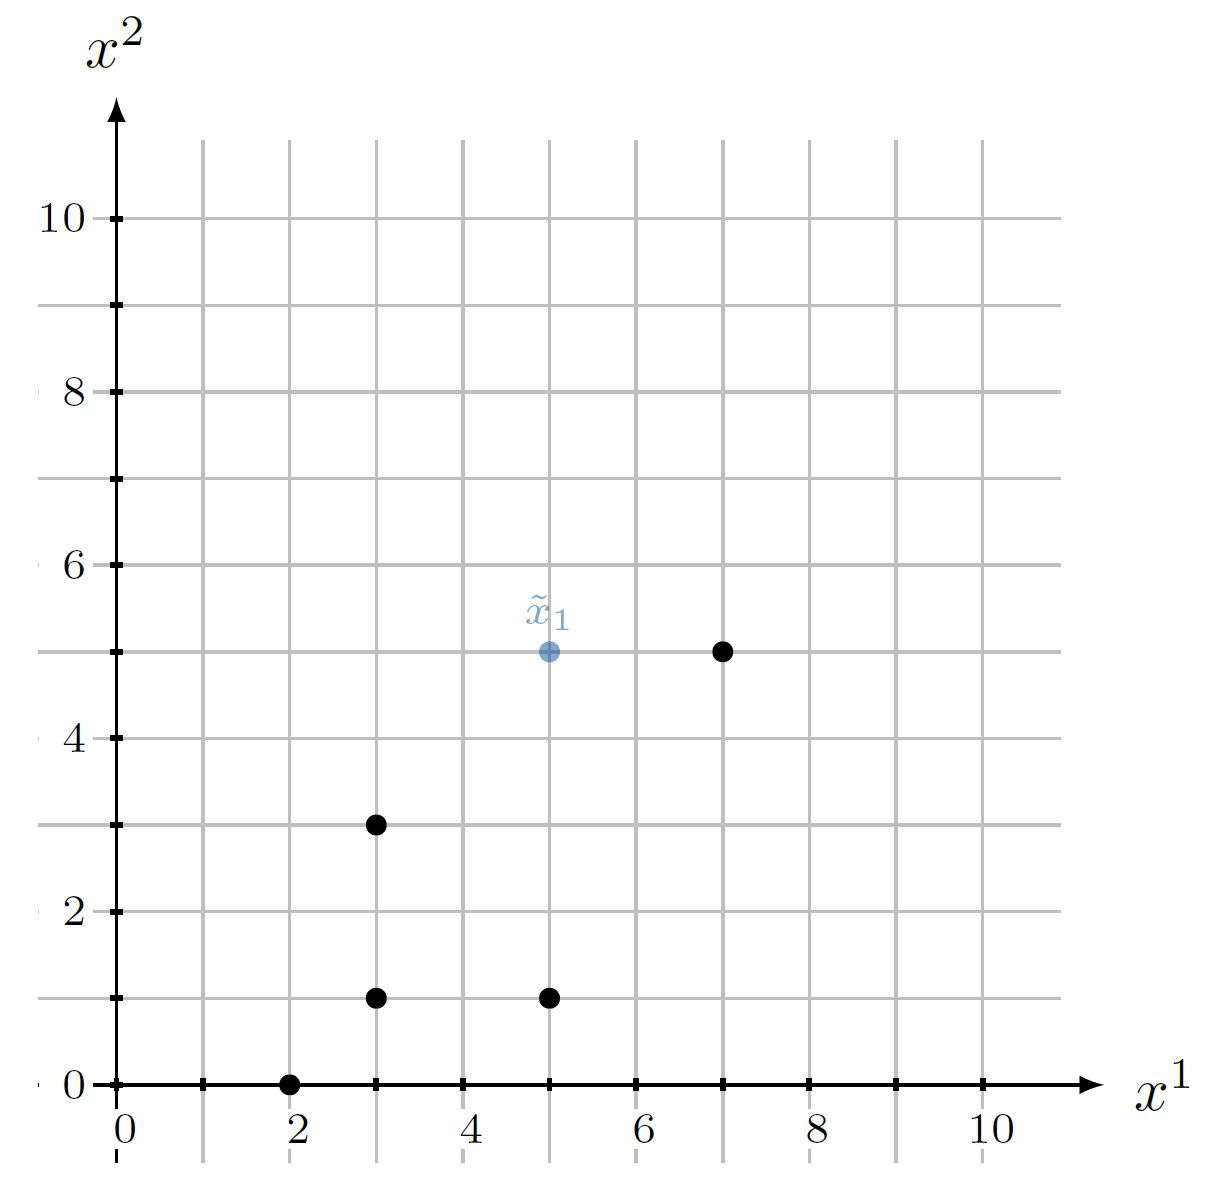
\includegraphics[scale=0.5]{figs/PCAbyHand1}
  \end{subfigure}
  \quad
  \begin{subfigure}[t]{0.4\linewidth}
      \centering
      \raisebox{3.5cm}{\begin{tabular}{@{}p{0.5cm}@{}cc}
        \toprule
        & $x^1$ & $x^2$\\
        \midrule
        \multirow{5}{*}{\rotatebox{0}{$X$}} & 2 & 0\\
        &3 & 1\\
        &7 & 5\\
        &3 & 3\\
        &5 & 1\\
        \midrule
        $\widetilde{X}$ & 5 & 5\\
        \bottomrule
        \end{tabular}}
  \end{subfigure}
\end{figure}

\medskip

\begin{enumerate}
  \item Principal component analysis requires a centered feature matrix. \blu{Find the vector of means $\mu=\begin{bmatrix} \mu_1 \\ \mu_2 \end{bmatrix}$ and compute the centered feature matrix $X_c$.}
  \item Writing $G_c= \begin{bmatrix} g_{11} & g_{12}\\ g_{21} & g_{22} \end{bmatrix} = X_c^\top X_c$, the first principal component $w_1=\begin{bmatrix}w_{11} \\ w_{12}\end{bmatrix}$ is given by the {\bf normalized} solution to the linear system $(G_c-{\bf I}_d\lambda_1)\cdot w_1 = 0$, where $\lambda_1$ is the largest solution to the quadratic equation $\chi(\lambda)=(\lambda-g_{11})(\lambda-g_{22})-g_{12}g_{21}=0$.\footnote{$\chi$ is called the \emph{characteristic polynomial} of $G_c$ and its roots are eigenvalues $\lambda$ whose corresponding eigenvectors $w$ solve the equation $G_cw = \lambda w$.} The second principal component $w_2=\begin{bmatrix}w_{21} \\ w_{22}\end{bmatrix}$ is given by the {\bf normalized} solution to the linear equation $w_1^\top w_2 = 0$. \blu{Compute the two principal components $w_1$ and $w_2$ (show your work).}
  \item The two principal components $w_1$ and $w_2$ form an orthonormal basis $W = \begin{bmatrix}w_{11} & w_{12}\\w_{21} & w_{22}\end{bmatrix}$ of $\mathbb{R}^2$. \blu{Represent the test point $\tilde{x}_1$ in this basis by performing an orthogonal projection $\tilde{z}_1 = \begin{bmatrix} \tilde{z}_{11} \\ \tilde{z}_{12} \end{bmatrix} = W(\tilde{x}_1-\mu)$ onto $w_1$ and $w_2$ (show your work).}

  \pagebreak

  \item We can now represent the PCA coordinate system in the orginal coordinate system. \blu{In the plot above, draw the two coordinate axes defined by $w_1$ and $w_2$, using $\mu$ as origin. Then visualize the PCA coordinates $\tilde{z}_1$ computed in 3.1.3 by drawing two lines between the test point and its orthogonal projections onto $w_1$ (given by $\begin{bmatrix} \tilde{z}_{11} \\ 0 \end{bmatrix}$ in the PCA coordinate system) and $w_2$ (given by $\begin{bmatrix} 0 \\ \tilde{z}_{12} \end{bmatrix}$ in the PCA coordinate system). Finally, use the visualization to read off the coordinates of $\begin{bmatrix} \tilde{z}_{11} \\ 0 \end{bmatrix}$ and $\begin{bmatrix} 0 \\ \tilde{z}_{12} \end{bmatrix}$ in the {\bf original} coordinate system, which can be interpreted as reconstructions of $\tilde{x}_1$. Report both reconstructions and their L2 reconstruction errors (show your work).}
  
   Note: If you want, you can draw the PCA coordinate system and the orthogonal projections directly in Latex; see the commented lines below this one in a5.tex for an example. Hand-drawn results will also be accepted.
   
%   \begin{tikzpicture}[scale=0.5, baseline=(current bounding box.center)]
%  \tkzInit[xmin=-0.9, xmax=10.9, ymin=-0.9, ymax=10.9]
%  \tkzGrid[color=grey]
%  \tkzDrawX[label = $x^1$, right = 4pt]
%  \tkzDrawY[label = $x^2$, above = 4pt]
%  \tkzDefPoint(2,0){P1}
%  \tkzDefPoint(3,1){P2}
%  \tkzDefPoint(7,5){P3}
%  \tkzDefPoint(3,3){P4}
%  \tkzDefPoint(5,1){P5}
%  \tkzDefPoint(5,5){test}
%
%  %Add coordinate axes and orthogonal projections here
%  %draw line
%  %\draw[dashed, color = red, opacity=0.5, line width= 0.5pt, line cap=round] (0,0) -- (5, 5);
%
%  \tkzDrawPoints(P1,P2,P3,P4,P5)
%  \tkzLabelPoint[above, blue, opacity=0.5](test){\scriptsize $\tilde{x}_{1}$};
%  \tkzDrawPoint[blue, opacity=0.5](test)
%
%  \tkzLabelX[orig=false, node font = \scriptsize, step=2]
%  \tkzLabelY[orig=false, node font = \scriptsize, step=2]
%\end{tikzpicture}


\end{enumerate}

\pagebreak

\subsection{Data Visualization}

If you run \verb|python main.py 3.2|, the program will load a dataset containing 50 examples, each representing an animal.
The 85 features are traits of these animals.
The script standardizes these features and gives two unsatisfying visualizations of it.
First, it shows a plot of the matrix entries, which has too much information and thus gives little insight into the relationships between the animals.
Next it shows a scatterplot based on two random features and displays the name of 15 randomly-chosen animals.
Because of the binary features even a scatterplot matrix shows us almost nothing about the data.

In {\texttt{encoders.py}}, you will find {a class named \texttt{PCAEncoder}}, which implements the classic PCA method (orthogonal bases via SVD) for a given $k$, the number of principal components. Using this class, create a scatterplot that uses the latent features $z_i$ from the PCA model with $k=2$.
Make a scatterplot of all examples using the first column of $Z$ as the $x$-axis and the second column of $Z$ as the $y$-axis, and use \texttt{plt.annotate()} to label the points corresponding to \verb|random_is| in the scatterplot.
(It's okay if some of the text overlaps each other; a fancier visualization would try to avoid this, of course, but hopefully you can still see most of the animals.)
Do the following:
\begin{asking}
	\begin{enumerate}
		\item Hand in your modified demo and the scatterplot.
		\item Which trait of the animals has the largest influence (absolute value) on the first principal component?
		\item Which trait of the animals has the largest influence (absolute value) on the second principal component?
    \end{enumerate}
\end{asking}

\pagebreak

\subsection{Data Compression}

It is important to know how much of the information in our dataset is captured by the low-dimensional PCA representation.
In class we discussed the ``analysis" view that PCA maximizes the variance that is explained by the PCs, and the connection between the Frobenius norm and the variance of a centered data matrix $X$. Use this connection to answer the following:
\blu{\enum{
\item How much of the variance is explained by our two-dimensional representation from the previous question?
\item How many\ PCs are required to explain 75\% of the variance in the data?
}}
Note: you can compute the Frobenius norm of a matrix using the function \texttt{np.linalg.norm}, among other ways. Also, note that the ``variance explained'' formula from class assumes that $X$ is already centred.

\pagebreak

\section{Very-Short Answer Questions}


\enum{
\item Assuming we want to use the original features (no change of basis) in a linear model, what is an advantage of the ``other'' normal equations over the original normal equations?
\item Describe the kernel trick in L2-regularized least squares in one sentence.
\item In class we argued that it's possible to make a kernel version of $k$-means clustering. What would an advantage of kernels be in this context?
\item What is the key advantage of stochastic gradient methods over gradient descent methods?
\item Which of the following step-size sequences lead to convergence of stochastic gradient to a stationary point?
\enum{
\item $\alpha^t = 1/t^2$.
\item $\alpha^t = 1/t$.
\item $\alpha^t = \gamma/t$ (for $\gamma > 0$).
\item $\alpha^t = 1/(t+\gamma)$ (for $\gamma > 0$).
\item $\alpha^t = 1/\sqrt{t}$.
\item $\alpha^t = 1$.
}
\item{Given discrete data $D$ and parameters $w$, is the expression $p(D|w)$ a probability mass function, a likelihood function, or both? Briefly justify your answer.}
\item{Why is it often more convenient to minimize the negative log-likelihood than to maximize the likelihood?}
\item How does the impact of the prior in MAP estimation change as we add more data?
\item What is the difference between a generative model and a discriminative model?
\item With PCA, is it possible for the loss to increase if $k$ is increased? Briefly justify your answer.
\item Why doesn't it make sense to do PCA with $k > d$?
\item In terms of the matrices associated with PCA ($X$, $W$, $Z$, $\hat{X}$), where would an ``eigenface'' be stored?
}


\end{document}
